\documentclass{article}

\usepackage{microtype}
\usepackage{graphicx}
\usepackage{booktabs}
\usepackage{hyperref}
\newcommand{\theHalgorithm}{\arabic{algorithm}}

% arXiv preprint: shows authors, drops the "under review" banner.
\usepackage[preprint]{icml2026}

\usepackage{amsmath}
\usepackage{amssymb}
\usepackage[capitalize,noabbrev]{cleveref}

\icmltitlerunning{What sets the ceiling on automated code audit}

\begin{document}

\twocolumn[
\icmltitle{What Sets the Ceiling on Automated Code Audit:\\
           the Auditor, its Rulebook, or the Specification?}

\begin{icmlauthorlist}
\icmlauthor{Zhaohe Dong}{ind}
\end{icmlauthorlist}

\icmlaffiliation{ind}{Independent researcher}
\icmlcorrespondingauthor{Zhaohe Dong}{dongzhaohe321418@gmail.com}

\icmlkeywords{code review, LLM critics, evaluation, preregistration}

\vskip 0.3in
]

\printAffiliationsAndNotice{}

\begin{abstract}
An automated auditor reads code it did not write and decides whether to block it. We ask how much
such an auditor catches and what decides the limit, against ground truth no model supplies: hidden
test suites executed by an interpreter. Holding the auditor, its instructions and its ground truth
fixed, and varying one thing at a time, we find the limit is set jointly by which model reads,
what its rulebook tells it to look for, and whether the benchmark's hidden suite asks a question
the specification answers.

Repeated independent reading saturates far below complete. Eight readings of the shipped
cross-vendor auditor reach $30.0\%$ union recall on defective increments $[20.0, 40.7]$, the
eighth reading adding $1.9$ points; twenty readings pooled across three auditor families reach
$48.2\%$ $[36.7, 60.0]$. Replacing the auditor with a stronger same-vendor model moves union
recall by $-26.4$ points $[-37.3, -15.6]$, a preregistered primary, so a stronger model is a worse
auditor here. Adding one sentence to the auditor's rulebook, telling it to look for what the
visible tests do not cover, moves flags by $+26.8$ points $[13.6, 40.4]$, the largest effect we
measure.

Much of what the auditor misses turns out to be failure the specification never determined. Under
a rule that asks whether the prose settles the hidden suite's expected value, two raters agree
that $44$ of the $57$ never-flagged defects are cases where it does not, reversing the same
instances' earlier classification and withdrawing a claim this work previously made. Where an
outside party had independently flagged one of these specifications as defective, our raters agree
on $9$ of the $11$ tasks that overlap.

Two cautions follow for work that reports critic and reviewer recall. First, a union-recall figure
is contingent on the matching rate on correct work: on a second substrate with three times longer
specifications the same auditor reaches more than twice the recall while flagging more than three
times as much correct code, and for that auditor the two substrates' false-positive intervals
never meet, so no reading count offers a matched comparison. Second, repeated reading buys
coverage in proportion to how much of the population sits near the auditor's decision boundary:
one auditor we measure returns an identical verdict on all $250$ instances across eight
independent readings while its replies, costs and latencies vary, so its union over $K$ readings
is flat by construction.

Every study was preregistered before its first model call, with hypotheses, intervals, kill
conditions and stopping rules fixed in advance; four preregistered hypotheses were killed by their
own rules. Every report was reviewed by a model from a different vendor with access to the raw
records, and the reviews are archived verbatim beside the results they judge.
\end{abstract}

\section{Introduction}
When a model writes code, reports a result or prepares a dataset, someone has to check it, and
increasingly that someone is another model. CrossAudit, the system every measurement here passes
through (\S\ref{sec:system}), is built on two rules for doing that. The model that audits must come
from a different vendor than the model that wrote the work, and what a deterministic check can verify
is verified by code, not by a model's opinion. An auditor of this kind reads work it did not write
and says whether to block it. We ask how much it catches, what decides the limit, and whether the
arrangement helps where checking matters most, in science.

A reviewer's score on a benchmark mixes at least four things: whether the model can see a defect,
whether it judges the defect worth blocking on, whether the benchmark's hidden tests define the
behaviour it would have to see, and how many times it is allowed to look. Work on critic models
improves the first two and reports the aggregate gain. We vary these factors one at a time where the
design allows it, against a truth no model supplies: a hidden test suite executed by an interpreter.
Some contrasts cannot be isolated: changing the reading model also changed its sampling, and the
role of the specification is a post hoc association.

\textbf{The limit on general-purpose code} (\S\ref{sec:ceiling}). Eight independent readings of the
shipped cross-vendor auditor reach 30.0\% union recall [20.0, 40.7] on defective code at 16.0\%
[10.1, 22.3] on correct code, and the eighth reading still adds 1.9 points, so returns diminish
without a plateau. A stronger same-vendor model, sampled differently, moves recall by $-26.4$
points [$-37.3$, $-15.6$] while flagging 3.3\% of correct code against 16.0\%, and the contrast
reverses sign under a weaker severity rule. One added rulebook sentence moves flags by $+26.8$ points
[13.6, 40.4] on an exploratory arm, at $+12.5$ points on correct code (an interval,
[$-3.6$, $+26.8$], that does not exclude zero), without measurably moving outcomes. Of 57 defects no
reading flagged, two model raters judge 44 to be behaviour the specification never determined (post
hoc). A recall figure is therefore contingent on auditor route, rulebook, decision rule and benchmark,
and is not portable without its false-positive rate.

\textbf{Auditing science} (\S\ref{sec:ai4s}). We then take the system into science, with one
preregistered study for each job a scientist would hand an auditor. On reported results, the
deterministic check that every number traces to its source flagged all 49 inconsistencies among a
report, its results file and its run log, and none of 25 results that were wrong consistently in all
three; the model auditor flagged 23 of those 25, 21 with a sound finding about the fault (post hoc).
On data, a validator written from the dataset's documentation and the auditor flagged different
faulty items, 92 and 65 of 140, and together 112, at the auditor's 2.9\% flag rate on clean data
(post hoc, counting only findings about the injected fault: 61 and 110). On scientific code with no
tests shown, reframing the task around the step rather than the whole problem cut the auditor's flags
on correct code from 68.7\% to 36.0\% and its recall from 87.7\% to 72.8\%, on the same programs.

\textbf{Contributions.}
\begin{itemize}\itemsep1pt
\item A measurement programme for an automated auditor's limit against executed ground truth, with
  union recall always reported beside the false-positive rate it cost: controlled changes to the
  number of readings and the rulebook, route comparisons that change model and sampling together,
  re-grading under decision rules, and a post hoc association with what the specification determines.
\item Evidence that no single factor fixes the limit on general-purpose code: each of these moves it,
  and a recall figure without its operating point does not transfer.
\item Operating points of an LLM auditor on scientific code, and comparisons of the LLM tier with
  deterministic verification on reported results (the shipped provenance checks and re-execution) and
  data (a documentation-derived validator), against executed or constructed ground truth. The tiers
  flag different faults, and each fails where the other does not.
\item A methodological finding: in all three science studies the auditor flagged defects in our own
  construction of items meant to be clean, so an evaluation of an auditor must establish that its
  clean items are clean by the auditor's standard, or its false-positive rate measures the evaluator.
\end{itemize}

\textbf{Preregistration and review.} Every study that made model calls was preregistered before its
first one, with hypotheses, intervals and stopping rules fixed in advance, and planned departures
recorded as numbered amendments. Two analyses were not registered in advance, and the paper names
both (Appendix~\ref{sec:method}). Four preregistered hypotheses were killed by their own rules, and
in the science studies one more. Every report was reviewed by a model from a different vendor with
access to the raw records, at between three and twenty-one rounds each, and the reviews are archived
verbatim. Section~\ref{sec:discussion} discusses what the measurements mean. The full method, results
and discussion are in Appendices~\ref{sec:method}--\ref{sec:discussion-full}, and the records, reviews
and the command that regenerates every figure are described in Appendix~\ref{sec:repro}.

\section{Method}

\subsection{Substrates and ground truth}

Both substrates are Python functions with executable hidden test suites, so every stratum,
recall denominator and false-positive population is decided by an interpreter and no model judges
any outcome. \textbf{Substrate 1} is HumanEval+ and MBPP+ (EvalPlus), whose median task is 41
words of prose and 6 lines of reference code, with the benchmark's base suite shown to the author
and its plus suite held back. \textbf{Substrate 2} is the standard-library half of BigCodeBench,
whose median task is 118 words and 41 lines. BigCodeBench ships one test class per task, so the
visible and hidden suites are separated here: two test methods chosen by a fixed seed are the
visible suite and all methods are the hidden suite, with the class run unmodified and told which
methods to execute. Tasks whose declared modules are unavailable in the frozen interpreter, or
whose reference solution fails its own suite there, are dropped before generation and counted.

Candidates are written by one generator shown the specification and the visible tests. A candidate
that passes the visible suite and fails the hidden one is a \textbf{defective} instance; one that
passes both is \textbf{correct}; one that fails the visible suite is discarded. Recall is measured
on the defective stratum and false positives on a sample of the correct stratum.

\subsection{The auditor and the estimand}

The auditor reads the specification, the visible tests and the candidate, and returns findings
with severities; an increment is blocked when any finding is graded BLOCKER. It never sees the
hidden suite. The estimand throughout is \textbf{union recall at $K$}: the fraction of defective
instances blocked by at least one of $K$ independent readings, averaged exactly over all
$\binom{K_{\max}}{K}$ subsets rather than by sampling. The matching quantity on the correct
stratum is the union false-positive rate. A union recall figure is reported only beside the
false-positive rate it cost.

\subsection{Statistics}

The independent unit is the instance and the resampling unit is the problem, because problems
recur across generation batches. Every rate carries a 95\% percentile bootstrap over whole problem
clusters (10{,}000 resamples, seeds fixed in each preregistration), with the Wilson interval
printed beside it and marked as too narrow. Paired contrasts carry an exact McNemar test and a
cluster-level sign-flip permutation test; where every discordant pair points one way the
percentile bootstrap's bound at zero is an artefact and an exact unconditional interval is quoted
instead. A saturation curve is summarised by a constrained exponential fit, and the fitted
asymptote is quoted only when the preregistered flattening bar is met; otherwise it is labelled an
extrapolation and the raw union at $K_{\max}$ is the number quoted. Counts of five or fewer are
quoted as counts.

\subsection{Preregistration and independent review}

Each study was preregistered before its first model call, fixing its population, hypotheses,
primary outcome, intervals, kill conditions, budget and stopping rule. Departures are numbered
amendments committed before the step they govern, each recording what was known at the time; where
an amendment followed an interim observation, the results say so and argue whether the change
could favour the hypothesis. Each report was then reviewed by a model from a different vendor with
read access to the raw records, asked to re-run the analysis, recompute the intervals
independently, and check every sentence against the records. No report entered this paper until
such a review ended in approval. Reviews are archived verbatim, including those that refused
approval, and several studies needed many rounds.

\section{Results}
The claims this paper defends, each with its interval and its label, are listed in
\texttt{CLAIMS.md}. A claim enters that file only after its report has passed an independent
review by a model from a different vendor with access to the raw records. Sections
\ref{sec:repeat}--\ref{sec:residual} draw only on reports that have passed such a review.
Section~\ref{sec:inreview} reports four studies that are still in that review; every number in it
carries the label \emph{in review}, and none of them is load-bearing for the claims above.
Rates carry the 95\% problem-cluster percentile bootstrap as the primary interval, with the Wilson
interval beside it where the source report gives one, because problems recur across generation
batches and an interval that treats instances as independent is too narrow. The coverage of that
bootstrap under this clustered design with 56 problem clusters has not been validated by
simulation, and every primary interval in this paper inherits that caveat.

Sixteen comparisons were computed in the study that carries the primary contrasts, under one
Bonferroni family with a threshold of $0.00313$. Where a $p$ value appears below, the exact
McNemar value and the cluster-level sign-flip permutation value are both given, because instances
within a problem are not independent and only the second respects that.

\subsection{Returns to repeated reading diminish short of complete}
\label{sec:repeat}

The shipped cross-vendor auditor reads an increment holistically and returns findings; an
increment is blocked if any finding is graded BLOCKER. Over eight independent readings of the same
110 defective instances, union recall rises from 10.7\% at one reading to 30.0\% [20.0, 40.7] at
eight. The eighth reading still adds 1.93 points, cluster [1.14, 2.78], against the flattening bar
of 1.0 points registered before the first model call. The bar was not met. The constrained fit
puts the asymptote at 31.5\%, but on our own registered criterion that figure is an extrapolation
and the raw union at eight readings is the number to quote. What the data support is diminishing
returns at the budget we could afford, not saturation: at 1.9 points per reading the curve was
still climbing when we stopped. That bar is also a function of where a family was stopped, so
families run only to $K = 4$ meet it more easily than families run to $K = 8$, and a curve that
meets it at a small $K_{\max}$ is making a weaker statement than one that meets it at a large one.
Twenty readings pooled across three auditor families reach 48.2\% [36.7, 60.0].

The price is measured on the same footing. Union false positives on 150 correct increments reach
16.0\% [10.1, 22.3] at eight readings, and the recall bought per point of false positive falls
monotonically as readings accumulate.

\begin{figure*}[t]
\centering
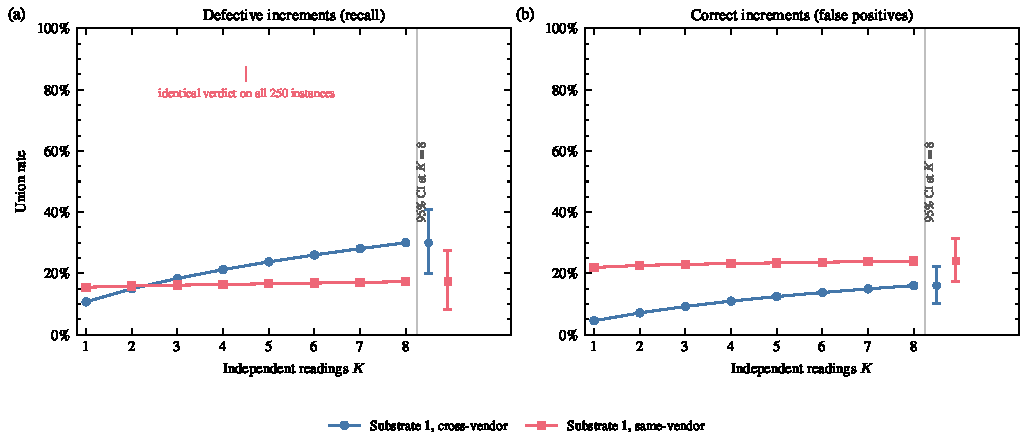
\includegraphics[width=\textwidth]{fig1_saturation.pdf}
\caption{\textbf{Returns to repeated reading diminish short of complete.} Union rate against the
number of independent readings $K$, for two auditor families on substrate 1. (a) recall on
defective increments; (b) false positives on correct increments. Bars at the right of each panel
give the 95\% problem-cluster bootstrap interval of each series at $K=8$, dodged in $x$ so
overlapping intervals stay separable. Neither curve meets the preregistered flattening bar: the
cross-vendor last-step gain is 1.93 points [1.14, 2.78] against a bar of 1.0, so neither is
described as saturating. The same-vendor route is sent temperature $0$ and the cross-vendor route
no sampling parameter at all, so the two unions are not equally free to rise with $K$
(\S\ref{sec:auditor}). A second substrate was plotted here until 2026-09-15 and is withdrawn
(\S\ref{sec:inreview}).}
\label{fig:saturation}
\end{figure*}

\subsection{Which model reads, and under which severity rule}
\label{sec:auditor}

Replacing the auditor with a stronger model of the generator's own vendor moved union recall at
eight readings by $-26.4$ points, cluster $[-37.3, -15.6]$: 4 of 110 against 33 of 110. Three
instances were flagged only by the new family and thirty-two only by the shipped auditor, at an
exact McNemar $p$ of $4.2 \times 10^{-7}$ and a cluster sign-flip $p$ of $2.0 \times 10^{-5}$.
This was a preregistered primary. Three things qualify what it means, all of them measured here
and none of them favourable to reading it as a statement about auditing ability.

First, the two auditors are not at the same operating point, which is the comparison this paper
elsewhere warns against. The stronger model flags correct code at 3.3\% [0.7, 6.7] against the
shipped auditor's 16.0\% [10.1, 22.3]. It blocks less of everything.

Second, the sign reverses under a weaker severity rule. Counting any finding rather than only
findings graded BLOCKER --- an exploratory rule, not preregistered --- the stronger model reaches
59.1\% [47.3, 70.6] on the defect population at 34.0\% [26.5, 41.7] on correct code, against the
shipped auditor's 34.5\% [23.6, 45.5] at 19.3\% [12.8, 26.3]. The ratio of those two rates --- a derived
point ratio we carry no interval for --- is 1.74 and 1.79 respectively, so nothing here shows one
family buying more recall per false positive than the other. The stronger model writes down
more of what is wrong and grades less of it as blocking. The $-26.4$ is a fact about severity
calibration.

Third, the two families are not sampled alike. The shipped cross-vendor route's capability card
does not permit a temperature, so no sampling parameter is sent and the route varies between
readings; the same-vendor route permits one and the layer sends temperature $0$, so that route is
near-deterministic. A union over near-deterministic readings cannot grow, and the two unions are
therefore not equally free to rise. They do not: over $K = 1$ to $8$ the cross-vendor family gains
19.3 points and the same-vendor family gains 3.0. At one reading the gap between them is $-10.1$
points, not $-26.4$; roughly two-thirds of the headline is the difference in how much each union
was permitted to grow. We regard this as the most serious limitation of the contrast, and
\S\ref{sec:limits} records what would be needed to remove it.

A third family argues the other way and belongs beside the headline. A high-reasoning model of the
cross-vendor family reaches 32.7\% [20.7, 45.0] union recall at four readings while flagging
10.7\% [5.9, 16.1] of correct code, dominating the shipped auditor on both axes at half the
readings. So the evidence does not support ``a stronger model is a worse auditor''. It supports
the narrower statement that this particular same-vendor model, at this severity calibration and
sampled at temperature $0$, blocks far less.

A same-vendor auditor of the generator's own size was worse than the cross-vendor one on these
instances by $-12.7$ points $[-25.0, -0.9]$ of union recall at eight readings, signed so that a
negative value favours the cross-vendor auditor. A study on a second substrate reverses that sign,
so this is reported as a measurement on this substrate rather than as a property of same-vendor
auditing.

\subsection{One rulebook sentence moves flags, and does not measurably move outcomes}
\label{sec:rulebook}

Adding a single rule to the auditor's constitution, telling it to find what the visible tests do
not cover, moved flags on the defect population from 10 of 56 to 25 of 56: $+26.8$ points, cluster
[13.6, 40.4], exact McNemar $p = 0.0003$, cluster sign-flip $p = 0.0009$. With the pooled
defect-and-correct flag contrast this is one of only two comparisons that clear the Bonferroni
threshold, and the two are the same effect seen twice.

The estimand is narrower than the sections above and must be read at its own scale. It is measured
on 56 instances from 41 problems, not the 110-instance defect population; it counts flags, not
union recall against the hidden suite; it is one reading, because every loop arm revises once, not
a union over eight; and it is exploratory, because the preregistration named outcome contrasts
rather than flag contrasts. For those reasons we do not compare its magnitude with the $-26.4$ or
the $+19.3$ of the preceding sections, which are union recall at $K=8$ over 110 instances. They
are different quantities on different populations.

Two costs travel with it. On correct code the same rule moved flags by $+12.50$ points [5.17,
21.82], so the sentence makes the auditor louder on both strata. And on the contrast that actually
isolates the rule --- the referent arm against the cross-vendor arm on hidden-suite pass rate after
one revision --- the effect is $+5.36$ points, cluster $[-0.89, +12.07]$, $p = 0.146$, which does
not exclude zero. The rule demonstrably moves what the auditor writes down. Whether that converts
into code that passes the hidden suite is not established, and since this paper argues elsewhere
that a flag is not a catch, that distinction applies to our own intervention first.


\subsection{Most of what the auditor missed is failure the specification never determined}
\label{sec:residual}

Fifty-seven of the 110 defective instances were flagged by no reading of any family. That is a
statement about twenty readings, not about detectability: if an instance is caught with
probability $p$ on each independent reading, twenty readings miss it with probability
$(1-p)^{20}$, which is still $98\%$ at $p = 0.001$ and $36\%$ at $p = 0.05$. Never flagged here
therefore does not mean never flaggable, and we use the residual as a population to characterise
rather than as a set of defects shown to be invisible.

The first classification of that residual asked whether the visible tests exercised the failing
input before it asked anything else. It called 46 of 57 unexercised edges, and an earlier draft of this paper
rested a claim on that.

Re-rating the same instances under a rule that asks first whether the specification's prose
determines the hidden suite's expected value reverses it. Two raters agree that 44 of 57 (77.2\%,
cluster [62.1, 91.1]) are cases where the prose does not settle the value, and that 2 of 57 are
cases where it does and the visible tests merely never built the input. The preregistered
condition for withdrawing ``the residual is mostly unexercised edge'' fires on both of its clauses,
and the claim is withdrawn. The interval is conditional on a category and has no committed
coverage simulation, so it is uncalibrated, as is every category-conditioned interval we report.

A classification that reverses when the order of its questions changes is, by itself, weak evidence
about the auditor, and the raters are not independent of it: one was the author, who wrote the
rubric and knew the earlier labels and which claim was at stake. Three things support the second
reading. The rubric was fixed before any label was written. The labels were committed before we
looked for outside evidence. And when a first pass was found to have carried instance identifiers
and a sheet name into the raters' view, the labelling was re-run with identities stripped and the
result held. Where an outside party had independently recorded that one of these specifications is
defective, in twelve MBPP tasks named in a paper written for another purpose, our raters agree on
9 of the 11 that fall inside our defect population, with both disagreements on the boundary that
paper's own ``incomplete'' category draws. That check is one-sided by construction: it can support
agreement where an outsider looked, and can bound nothing about the rate.

\subsection{Four studies in review, and what their reviews found}
\label{sec:inreview}

Four further studies had reported when this paper was written, and all four were refused quotation
by their independent reviews on the same day. We report that outcome rather than their numbers,
because two of the refusals bear on how far the results above reach.

\textbf{A second substrate, withdrawn.} This paper reported a second benchmark until its review
refused quotation, and we then confirmed the reason ourselves: the visible-test text shown to the
auditor \emph{and} to the generator was sliced out of its test class without the class header, so
it failed to parse on all 300 tasks, while scoring executed the intact class. Both models read
invalid Python on every task of that substrate. An auditor shown a broken test file can return a
finding about the file rather than about the candidate, which raises the flag rate on both strata at
once and so inflates recall and false positives together; the finding texts were not archived, so no
reading can be reclassified after the fact. The extraction is fixed and the study is registered for
a re-run whose numbers we will report whichever way they move.

\textbf{A prospective test of the residual, withdrawn.} We constructed a population of injected
defects intended to make specification-determinedness hold by construction. Review established that
it does not: the filter we registered to recover each edit's first failing hidden input was
implemented as a check that the injector had written a non-empty string, and no check connects the
quoted specification text, the named input class, the witness and the actual failure. What the
population contains is small edits that survive a sparse visible suite and fail a hidden one, and a
preregistered probe separates them from natural code at 96.7\%. The auditor does block them far
more often than it blocks the natural residual, but the two populations differ in more than the
property we meant to isolate, so this is not the prospective test of \S\ref{sec:residual} and we
do not offer it as one.

\textbf{Two others.} A study of what a flag is worth, and a study of whether a changed rulebook
moves a second vendor's family, were both refused for overstating what their measurements
establish; their corrections do not change any number quoted above.

We report these outcomes because a paper that makes evidentiary discipline its method should show
the gate rejecting its own work, not only passing it. None of the numbers in
\S\ref{sec:repeat}--\S\ref{sec:residual} depends on any of these four studies.

\subsection{What follows for a recall number}

Taken together, the results above say an audit recall figure is a joint property of the auditor
and its material. It moves with which model reads, with what the rulebook tells it to look for,
and with whether the benchmark's hidden suite asks a question the specification answers. It also
moves with the severity threshold at which a finding becomes a block, and with how the route is
sampled, neither of which is usually reported.

\section{Discussion}
\label{sec:discussion}

\textbf{A recall number is an operating point.} Recall and false positives move together with any
severity threshold, and a critic can be tuned to any recall by blocking more. On general-purpose code
the same auditor sits at different points under different decision rules, repetition buys recall at
a roughly constant price in false positives, and pooling families buys coverage at a higher one. On
scientific code the operating point also moved with what the task named as the deliverable. A recall
figure quoted without its false-positive rate, its rulebook, its decision rule and its task framing
does not carry to another setting.

\textbf{What the science studies add.} They give the science profile's design rule (the model names
evidence, code verifies it) an empirical reading and a boundary. On results, number$\to$source
verified every inconsistency between a report, its results file and its log, and could not see a
result that was wrong consistently; the model, by recomputing, flagged 23 of 25 such fabrications. On
data, a validator written from the card caught what a rule can state and missed what needs reading
across columns and units, which the model caught in 18 of the 28 such items the validator missed.
Where both tiers ran, the deterministic one flagged no clean item and the model carried the errors;
on data the union was better than either part, and on results the model's flags already contained
the profile's, whose findings its prompt carried. Neither study shows that the model tier scales: the
artefacts were small, the model's fabrication findings are hand calculations (several wrong), and it
missed every fault that needs comparison across many rows. A model reading is a useful second tier
where the artefact fits in the reader's working memory, not a substitute for executing the code or
computing over the data.

\textbf{Clean items must be clean by the auditor's standard.} In all three science studies the auditor
flagged defects in our own construction: a card and file that named a column differently, a file
outside the audited scope, a report claiming a run no file performed, a provenance sentence false for
inputs passed as literals, a unit label contradicting the code's documentation, and a task that named
the whole problem when one step was delivered. Each was a correct flag on an item we had built as
clean. We caught two in pilots, one when every verdict came back as an escalation, and the rest only
by reading every flag on a clean item, which the registrations required. Without that reading, the
false-positive rate would have measured the evaluator.

\textbf{Limits.} The auditor families are not sampled alike, which bounds every cross-family union
contrast, and no family was compared at a matched false-positive rate. Primary intervals are
problem-cluster bootstraps whose coverage was simulated only for single rates. Every rating was made
by a model, one of them the agent that designed the studies; no human rated anything. The reviewer of
every report is also one of the measured families. The science studies use one benchmark or four
tables each, synthetic faults, small artefacts and one generator. The full limits, and the
experiments that would remove them, are in Appendices~\ref{sec:discussion-full} and~\ref{sec:limitations-full}.

\section{Related work}

\textbf{Critics and repeated reading.} Trained critic models catch more bugs in model-written code
than unaided humans and hallucinate some \citep{mcaleese2024critics}; aggregating several review
passes raises review F1 on real pull requests \citep{zeng2025swrbench}; and coverage under repeated
sampling grows roughly log-linearly with the number of samples over four orders of magnitude
\citep{brown2024monkeys}. The natural-defect setting, the
precision cost of a louder critic and the diminishing returns of repeated sampling are therefore known.
What we add is narrow on this axis: the union of independent readings as an instrument for locating
a limit, ground truth supplied by an interpreter, and the false-positive rate beside every recall
figure.

\textbf{Who audits whom.} Self-correction without external feedback does not reliably improve
reasoning \citep{huang2024selfcorrect}, and model judges prefer their own generations, harmfully on
instances they get wrong \citep{chen2025selfpreference}. Our same-vendor arms are the code-audit case
of that literature; because routes differ in model, operating point and sampling, we report their
contrasts as contrasts between routes, not as self-preference.

\textbf{What the hidden suite decides.} EvalPlus rebuilt HumanEval and MBPP with larger suites
\citep{liu2023evalplus}; models collapse onto one reading of an underspecified task, and twelve MBPP
tasks were named as such by hand \citep{richter2026collapse}. Generated tests err mostly in the
expected value \citep{xiong2023testing}, and generated oracles tend to capture what a program does
rather than what was intended \citep{konstantinou2024oracles}. Our claim is the auditing counterpart:
where the prose does not fix the value, a recall number computed against that suite measures the
benchmark as much as the auditor. Consensus filters for generated tests
\citep{taherkhani2026consistency, xu2025consensus} and self-consistent errors \citep{tan2025consistent}
bear on one of our appendix studies (Appendix~\ref{sec:related-full}).

\textbf{Auditing scientific work.} On manuscripts, no model exceeds 21.1\% recall or 6.1\% precision
on errata-grade errors and repeated runs rarely rediscover the same errors \citep{son2025spot}; the
best models detect 46.7\% of real paper--code discrepancies \citep{baumgartner2026scicoqa}. An LLM
auditor of AI-scientist projects detects hand-labelled pitfalls far better with logs and code than
with the paper alone \citep{luo2025pitfalls}; pattern-based linting targets methodology bugs in
scientific Python \citep{samsonau2026scicodelint}; cleaning agents find row-level errors in corrupted
tables and miss errors spanning rows \citep{bendinelli2025cleaning}; and simulation code can run and
still solve the wrong equations \citep{song2026moose}. SciCode supplies scientist-written tests
\citep{tian2024scicode}, and an expert audit of it found many specifications and tests that reject
correct solutions \citep{hu2026scicodeverified}; reproduction benchmarks ask agents to recover
reported results \citep{siegel2024corebench}. On constructed statistical workflows, LLM reviewers
detect planted flaws almost always but flag 17--50\% of correct scripts \citep{chelate2026replicationtrap},
and \citet{luo2025pitfalls} already report both true- and false-positive rates. Scientific auditing and paired
operating points are therefore not new. What we add is this measurement programme applied to
scientific code, and the comparison of the model tier with deterministic verification on reported
results and data, which we did not find in prior work.

\textbf{Preregistration.} Preregistration of evaluation protocols is beginning to appear in machine learning
\citep{vaccaro2026prereg, thomas2026phacking}; we count our use of it as method, not contribution.


\section*{Reproducibility and claims}
The claims this paper is willing to defend, each with the interval and the label its source report
gives it, are listed in \texttt{CLAIMS.md} in the accompanying repository, together with the
claims the evidence does not support. Every preregistration, every numbered amendment, every
report and every independent review is archived there verbatim.

\bibliography{paper}
\bibliographystyle{icml2026}

\end{document}
